\section{Multilingual fairness}
\label{sec:multilingual}

Does the system protect consumers equally whatever the language of their contract? The groups are the languages of the multilingual evaluation set (Section~\ref{sec:data-multi}): the Terms of Service of the same 10 companies in English, German, Italian and Polish. English, the language of the training data and of the knowledge base, is the reference group. All language models in this section are Qwen3.6-27B (Section~\ref{sec:openweight}), so that one model is compared across languages. We first check that the replication reproduces the English results.

\subsection{Replication with the open-weight model}

Every experiment on UNFAIR-ToS was repeated with Qwen3.6-27B, with the same prompts, knowledge base, selection rule and evaluation (Table~\ref{tab:replication}).

\begin{table}[ht]
\centering\small
\caption{gpt-4.1-mini and Qwen3.6-27B on the UNFAIR-ToS test set: macro-F1 / precision / recall.}
\label{tab:replication}
\begin{tabular}{@{}lcc@{}}
\toprule
System & gpt-4.1-mini & Qwen3.6-27B \\
\midrule
Plain LLM & 64.2 / 41.3 / 93.6 & 64.2 / 35.9 / 97.1 \\
RAG, no gate & 71.3 / 55.0 / 93.0 & 71.8 / 53.4 / 95.9 \\
RAG examples only, no gate & 75.3 / 71.2 / 86.0 & 77.6 / 67.2 / 93.0 \\
\textbf{RAG + gate (main)} & \textbf{79.4 / 82.3 / 83.7} & \textbf{79.0 / 79.7 / 84.3} \\
RAG examples only + gate & 78.9 / 83.7 / 80.8 & 80.2 / 83.0 / 82.6 \\
\bottomrule
\end{tabular}
\end{table}

Every finding holds with a very different model.
\begin{itemize}
  \item \textbf{Same gate setting.} The selection procedure independently chooses the same gate ($k=8$, $m=3$).
  \item \textbf{Same ablation pattern.} Legal knowledge alone gives the lowest scores on validation, examples alone beat the full RAG, and the gate lifts both.
  \item \textbf{Same main result.} The two main systems differ by 0.4 macro-F1 (95\% interval $-2.2$ to $+1.4$). Against Legal-BERT, retrained on the cluster (82.8 $\pm$ 1.0 macro-F1, reproducing the earlier result), the gap is not significant for any seed.
  \item \textbf{Same picture for the explanations.} Grounding does not separate right from wrong (93\% against 96\% consistent legal evidence without the gate), while expert precedents do (44\% against 86\%). The faithfulness results also match (Section~\ref{sec:explanations}).
\end{itemize}
The English experiments took 3\,h\,50\,min on one GPU (about 14,800 requests, 32 in parallel).

\subsection{Fairness by language}

For each system and language we compute the criteria of Section~\ref{sec:background}:
\begin{itemize}
  \item recall of unfair sentences (equality of opportunity);
  \item false-alarm rate (with recall, equalized odds);
  \item precision (conditional use error);
  \item share of flagged sentences (statistical parity).
\end{itemize}
Each language is compared with English in two ways. The first is the \textbf{ratio} of the rates, where, following the AEQUITAS convention seen in the course~\citep{slides_aequitas}, a ratio between 0.8 and 1.25 counts as parity. The second is the \textbf{difference}, with a 95\% bootstrap interval obtained by resampling each language independently. Table~\ref{tab:fairness} and Figure~\ref{fig:languages} give the results.

\begin{table}[ht]
\centering\small
\caption{Recall, false-alarm rate and macro-F1 per language (en / de / it / pl) on the multilingual evaluation set. LLM systems: Qwen3.6-27B.}
\label{tab:fairness}
\begin{tabular}{@{}lccc@{}}
\toprule
System & Recall & False-alarm rate & Macro-F1 \\
\midrule
Legal-BERT (English only) & 72.6 / 0.0 / 0.0 / 0.0 & 1.3 / 0.0 / 0.0 / 0.0 & 76.0 / 10.5 / 10.6 / 10.6 \\
TF-IDF + SVM (English only) & 55.3 / 0.5 / 0.0 / 0.0 & 1.0 / 0.0 / 0.0 / 0.0 & 66.7 / 11.6 / 10.6 / 10.6 \\
kNN vote (bge-m3) & 70.3 / 64.4 / 69.4 / 68.1 & 3.4 / 4.1 / 3.5 / 3.4 & 65.5 / 58.9 / 61.6 / 61.2 \\
Plain LLM & 95.9 / 91.8 / 92.1 / 92.0 & 13.3 / 13.7 / 14.2 / 12.4 & 64.7 / 64.0 / 62.1 / 63.7 \\
RAG, no gate & 90.4 / 86.3 / 88.2 / 87.0 & 7.2 / 7.3 / 6.6 / 6.6 & 73.1 / 69.8 / 70.4 / 69.5 \\
RAG + gate & 77.2 / 72.1 / 75.1 / 73.9 & 2.1 / 2.9 / 2.1 / 2.1 & 74.4 / 68.3 / 69.8 / 70.7 \\
\bottomrule
\end{tabular}
\end{table}

\begin{figure}[ht]
\centering
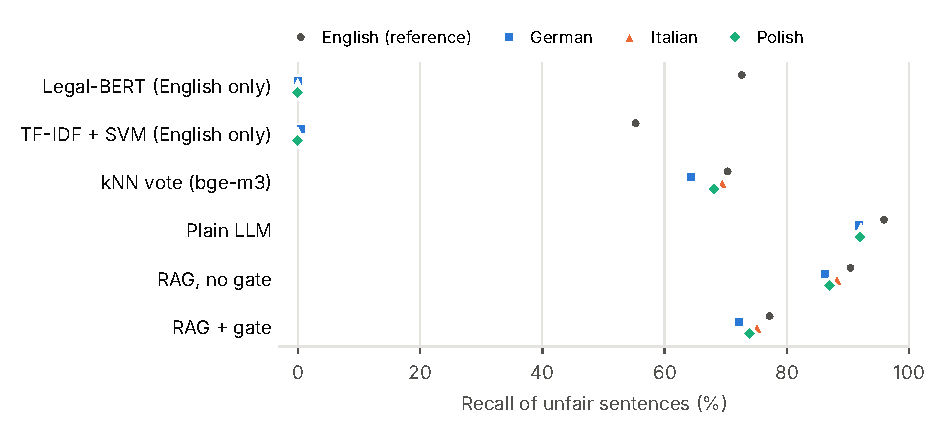
\includegraphics[width=0.82\textwidth]{recall_by_language.pdf}
\caption{Recall of unfair sentences per language. The English-only models find almost nothing outside English; the multilingual systems stay close to English in every language.}
\label{fig:languages}
\end{figure}

\begin{itemize}
  \item \textbf{English-only models give no protection in the other languages.} Legal-BERT and TF-IDF find 55--73\% of the unfair clauses in English and almost none in German, Italian and Polish: a complete violation of equality of opportunity. Their false-alarm rates are ``equal'' only because they flag nothing, which shows why one fairness criterion alone is not enough.
  \item \textbf{The multilingual systems protect the four languages about equally.} For the kNN vote and the three LLM systems, every recall ratio lies in the parity band, from 0.92 to 0.99. No difference from English is significant at 5\%, whether in recall, false alarms, precision or macro-F1.
  \item \textbf{One ratio falls outside the band without a real gap.} RAG + gate flags 2.9\% of the fair German sentences against 2.1\% in English, a ratio of 1.37. The difference, +0.8 points (interval $-0.1$ to $+1.7$), is not significant: ratios of small rates are unstable, so ratio and difference must be read together.
  \item \textbf{German has the lowest recall for every multilingual system}, 4--6 points below English. No single gap is significant, but the pattern is systematic and deserves a larger test set.
  \item \textbf{The gate keeps the parity.} It cuts the false alarms from about 7\% to about 2\% in every language, at the cost of 13--14 points of recall, the same trade-off as in English.
\end{itemize}

The English scores are lower than on UNFAIR-ToS (for example 76.0 against 82.8 macro-F1 for Legal-BERT), because these are contracts of other companies, written later. Languages should therefore be compared within this table only.

\paragraph{Mitigation.} Our proposal planned to compare two mitigation strategies: translating contracts into English before classifying them (pre-processing, in the terms of the course~\citep{slides_mitigation}), and multilingual retrieval. The results make the comparison unnecessary for our systems. A multilingual embedding model with a multilingual language model already reaches parity, so there is no gap left to close. Translation would matter only for the English-only models, and for them it would mean replacing their input pipeline with a second AI system whose errors would then need their own fairness analysis.
